% !TeX root = ../main.tex
% Supplementary materials moved from ch5/papers/RLHF/main.tex.
\chapter[Supplementary materials for Study 5.3]{Supplementary materials for Study 5.3: caregiver feedback}
\label{app:feedback}
\begingroup
\graphicspath{{ch5/papers/RLHF/}}

\section{Additional analyses}
\label{app:analyses}

\begin{center}
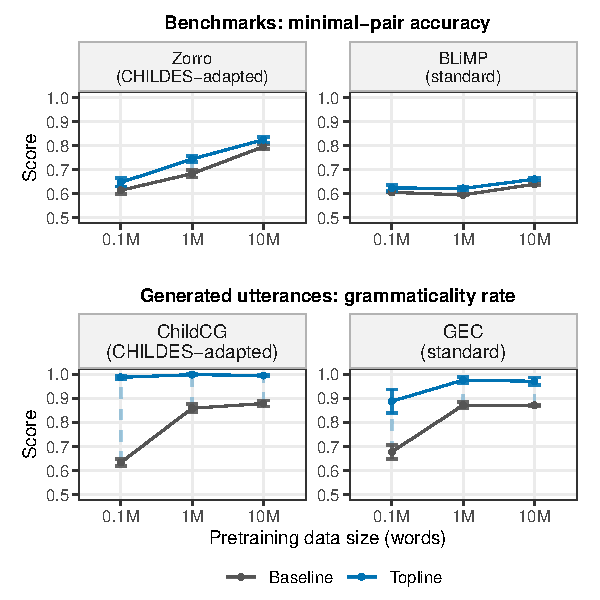
\includegraphics[width=0.7\textwidth]{figures/figureA_baseline_topline_scale_mixed_sources_new.pdf}

\captionof{figure}{
Baseline and Topline performance across pretraining scales. The top row reports minimal-pair benchmark accuracy for Zorro and BLiMP. The bottom row reports grammaticality of generated utterances, using the ChildCG or GEC-based metric. Points show means across training runs (after averaging generation-based measures over generation seeds). Error bars show $\pm 1$ standard deviation across those runs.
}
\label{fig:topline}
\end{center}

\begin{figure*}[t]
    \centering
    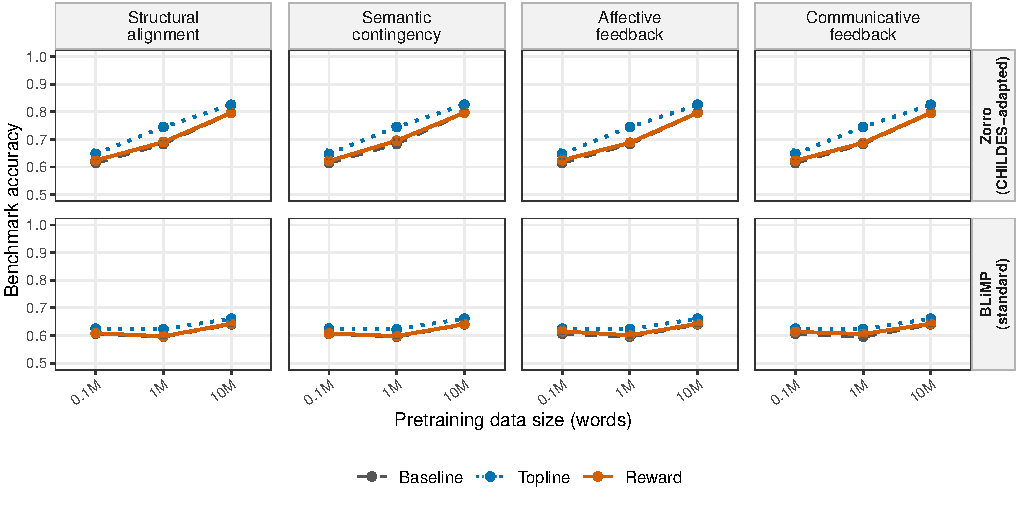
\includegraphics[width=\textwidth]{figures/figureB_benchmark_scale_trajectories.pdf}
    \caption{
    Benchmark performance across pretraining scales for each reward family.
    Rows show Zorro and BLiMP minimal-pair accuracy; columns show the four empirical reward families.
    Within each panel, the baseline and topline trajectories are repeated to make the reward trajectory directly comparable at each scale.
    Means are computed across training runs. Error bars show $\pm 1$ standard deviation across those runs; generation seeds do not provide independent model replications for fixed minimal-pair evaluation.
    }
    \label{fig:benchmark_reward_scale}
\end{figure*}


\begin{figure*}[t]
    \centering
    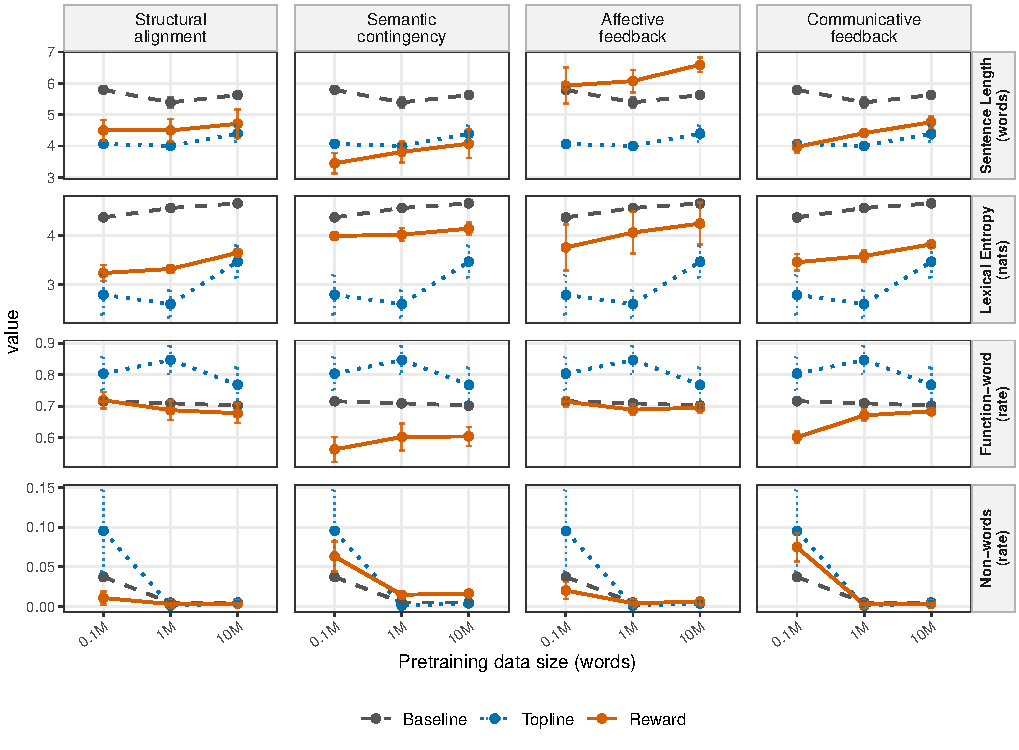
\includegraphics[width=\textwidth]{figures/figureD_covariates_scale_trajectories.pdf}
    \caption{
    Properties of generated utterances: Sentence length, pooled lexical entropy, function-word density, and rate of non-words.
    Points show means for each reward across training seeds, with error bars indicating $\pm 1$ standard deviation across these seeds.
    Within each panel, baseline and topline trajectories are repeated to make the reward trajectory directly comparable at each scale.
    }
    \label{fig:covariates_reward_scale}
\end{figure*}

\clearpage


\section{Example generations}
\label{sec:rlhf_examples}
\begin{table}[H]
\vspace{1em}
\centering
\scriptsize
\setlength{\tabcolsep}{3.5pt}
\renewcommand{\arraystretch}{1.18}

\begin{tabular}{
p{0.12\textwidth}
p{0.12\textwidth}
p{0.30\textwidth}
>{\columncolor{gray!15}}p{0.38\textwidth}
}
\toprule
Reward type &  & ChildCG = 1 (classified grammatical) & ChildCG = 0 (classified ungrammatical) \\
\midrule

\textbf{Baseline} &  &


\textit{you want to look at some more pictures?}

\textit{oh, is that what it looks like?}

\textit{it is a big boy now isn't it?}

\textit{have you not any other little boys?}
&
\textit{this piece of cake?}

\textit{because you can see mummy's poorly sick.}

\textit{the dog is saying.}

\textit{he is the name of the little girl.}
\\
\midrule

\textbf{Topline} &  &
\textit{what are you doing?}

\textit{there is a horse.}

\textit{that is a girl.}

\textit{are you going back?}

\textit{that is a chair.}

\textit{what is that one?}

\textit{i will put it there.}

\textit{what did we do with the barn?}
&
\textit{why is that side?}
\\
\midrule

\begin{tabular}[t]{@{}l@{}}\textbf{Structural}\\\textbf{Alignment}\end{tabular} & &
\textit{so that is a duck.}

\textit{he is a turtle.}

\textit{you are a good boy.}

\textit{i am a monkey.}
&
\textit{how many trucks in the sky.}

\textit{come down the street.}

\textit{we are a good boy.}

\textit{can't find it.}
\\
\midrule

\begin{tabular}[t]{@{}l@{}}\textbf{Semantic}\\\textbf{Contingency}\end{tabular} & &
\textit{yes that is a doggie.}

\textit{well it is a boat.}

\textit{there is an elephant.}

\textit{yes a banana puppy.}
&
\textit{where is baby sheep?}

\textit{what is big truck?}

\textit{he a lion.}

\textit{a big flower red.}
\\
\midrule

\begin{tabular}[t]{@{}l@{}}\textbf{Affective}\\\textbf{feedback}\end{tabular}
&  &
\textit{and then i will put it in it.}

\textit{i will put it over here if i put it in there.}

\textit{we have to wash her hair first okay?}

\textit{we will shall we put it all together?}
&
\textit{if i do it and then we can do it and put it in?}

\textit{now i will have to clean this with your room won't you?}

\textit{want mama do it?}

\textit{because your teeth i am watching this picture aren't they?}
\\
\midrule

\begin{tabular}[t]{@{}l@{}}\textbf{Communi-}\\\textbf{cative}\\\textbf{feedback}\end{tabular}
& Acknowledge-\newline ment &
\textit{they are called flowers.}

\textit{that is a gold straw.}

\textit{and that is the baby.}

\textit{you have a pink one on there.}
&
\textit{have to use your spoon and pretend.}

\textit{you will use them ones with this bits.}

\textit{all day and then the is warm.}

\textit{but two grey stars.}
\\
\cmidrule(lr){2-4}

& \begin{tabular}[t]{@{}l@{}}Clarification\\request\end{tabular} &
\textit{i don't know.}

\textit{can you see it?}

\textit{can't you?}

\textit{mhm, it is.}
&
\textit{look at that isn't it?}

\textit{look it, there is it?}

\textit{see you shouldn't?}

\textit{there doesn't.}
\\

\bottomrule
\end{tabular}

\caption{
Examples of utterances generated by RL-fine-tuned models at the 10M-word scale (generation was qualitatively similar at the 1M-word scale).
Examples are organized by reward types. Unshaded cells show utterances that were classified as grammatical by ChildCG, while shaded cells show utterances classified as ungrammatical.
}
\label{tab:sampled_childcg_examples}
\end{table}



\clearpage
\section{Automatic labeling of rewards}
\label{sec:rlhf_annotation}

We automatically annotated caregiver feedback signals in child-caregiver conversations and used these annotations to supervise reward model training (see Appendix~\ref{sec:rlhf_training}).

\subsection*{Communicative feedback}

\noindent \textbf{Clarification requests} 
Clarification requests were identified using a DeBERTa-v3-xsmall classifier fine-tuned on manually annotated caregiver responses in CHILDES, following prior work \citep{nikolaus_fourtassi_2026}.

\noindent \textbf{Acknowledgements} To identify caregiver acknowledgements, we relied on the feature-based algorithm described in \citet{nikolaus_communicative_2023a}, which was specifically designed for CHILDES data and combined common keywords (e.g., ``okay'', ``alright'', and ``yeah'') as well as repetition ratios capturing repetition-based acknowledgements (e.g., ``It isn’t very nice, is it?'' – ``It isn't.''). 
%When evaluated on CHILDES data, the algorithm achieved an accuracy of 0.82.

\subsection*{Structural Alignment}

%Structural alignment  and semantic contingency. We annotated child--caregiver alignment using a dedicated pipeline applied to cleaned child utterances and immediately following caregiver responses. 

Following previous research \cite{dale_unraveling_2006, fernandez_quantifying_2014}, a child structure was defined as a POS bigram. We used spaCy (\texttt{en\_core\_web\_sm})\footnote{\url{https://huggingface.co/spacy/en_core_web_sm}} to tag each child utterance and caregiver response for part-of-speech (POS), excluding punctuation and empty tokens. Caregiver alignment was computed as a normalized score of bigram reuse: the size of the intersection between the child and caregiver POS-bigram sets divided by the size of the larger set. This overlap is symmetric in the two sets; the child-to-caregiver direction comes from their order in the recorded exchange. It does not distinguish a caregiver recast from other responses containing the same POS bigrams.

\iffalse
\[
\mathrm{Align}_{syn}(c,a) =
\frac{|B_{POS}(c) \cap B_{POS}(a)|}
{\max(|B_{POS}(c)|, |B_{POS}(a)|)}.
\]
When both utterances contained no POS bigrams, the score was set to 1; when only one utterance contained POS bigrams, the score was set to 0. This score was used as the structural alignment reward.
\fi

\subsection*{Semantic Contingency}

Following previous research \cite[e.g.,][]{fusaroli_caregiver_2023, foushee2022getting}, semantic contingency was computed using sentence embedding similarity. Here, we used \texttt{all-MiniLM-L6-v2}\footnote{\url{https://huggingface.co/sentence-transformers/all-MiniLM-L6-v2}} to encode the child utterance and caregiver response. We computed the cosine similarity between the two embeddings, and clipped the resulting score to the $[0,1]$ range.

\iffalse
\[
\mathrm{Align}_{sem}(c,a) =
\mathrm{clip}_{[0,1]}
\left(
\cos(\mathbf{e}_c, \mathbf{e}_a)
\right).
\]
This semantic similarity score was used as the semantic contingency reward. The same pipeline also computed lexical unigram and bigram overlap based on spaCy lemmas, but these lexical scores were not part of the main reward families analyzed in the present paper.
\fi

\subsection*{Affective feedback}

We annotated affective properties of caregiver responses using \texttt{roberta-base-go\_emotions}.\footnote{\url{https://huggingface.co/SamLowe/roberta-base-go_emotions}} The model was applied to adult responses only. For each caregiver utterance, the classifier returned scores for several emotion labels. We used the probabilities for emotions related to supportiveness, approval, and warmth.

%was computed as the mean of admiration, approval, caring, optimism, and pride; engagement as the mean of curiosity, excitement, amusement, and desire and warmth as the mean of caring, love, gratitude, and joy. We additionally retained individual probabilities for approval, curiosity, and caring. Empty or missing caregiver responses were assigned zero scores for all affective dimensions. 

%In the main experiments, affective feedback was based on warmth, supportiveness and approval. 




\section{Baseline and reward-model training}
\label{sec:rlhf_training}

\subsection*{Baseline models}
For the input-based baselines, we trained a small GPT-2-style causal language model on caregiver utterances only. The model used 2 hidden layers, 8 attention heads, and a hidden size of 512. We trained a word-level tokenizer on the training data, retaining words that appeared at least twice and capping the vocabulary at 5,000 types. Models were optimized with the standard GPT-2 causal language-modeling objective using AdamW and a batch size of 256. For each data scale, we held out 10\% of the data for validation and used validation loss for early stopping and checkpoint selection. To assess the effect of input size, we trained models on three amounts of caregiver language: 0.1M, 1M, and 10M words. Each condition was run with three different random seeds.

\subsection*{Reward models}

For each of the four caregiver feedback dimensions above, we train a reward model that maps a child utterance to the corresponding valence of the caregiver response, as annotated using the procedures described in Appendix~\ref{sec:rlhf_annotation}.

%The grammaticality topline is trained in the same way, using the ChildCG annotations of \citet{nikolaus_automatic_2024} as target labels.


All reward models share the same pre-trained model:
\texttt{microsoft/deberta-v3-xsmall} \citep{he_debertav3_2022}, which we fine-tune using linear regression layer and a mean squared error (m.s.e.) loss to predict the target reward for a given utterance.


\iffalse

with a single-logit sequence-classification head.  Given a tokenized utterance $u$, the model outputs a logit $z_\phi(u)$ and we apply a sigmoid, $\hat{y}_\phi(u) = \sigma(z_\phi(u))$.  The model is trained with a mean-squared error objective against the (continuous or binary)
target valence $y(u) \in [0,1]$:
\begin{equation}
    \mathcal{L}(\phi) \;=\; \mathbb{E}_{(u,y)\sim\mathcal{D}}
    \big[\, ( \sigma(z_\phi(u)) - y )^{2} \,\big].
\end{equation}
We deliberately use a regression objective rather than a pairwise preference loss, because the underlying caregiver-behavior annotations are intrinsically scalar (e.g.\ POS-bigram overlap, sentence-similarity, or emotion-classifier probabilities) rather than preference comparisons.
\fi

The empirical reward models are trained on CHILDES child--caregiver conversation pairs, with one row per child utterance and its immediately following caregiver response. The grammar-targeted reference instead uses BLiMP and Zorro labels, as described below.
We split the data into 90\% training and 10\% held-out evaluation with a fixed random seed.  
We used the AdamW optimizer with an initial learning rate of $1.41 \times 10^{-5}$, a batch size of 128, and early stopping based on MSE on the held-out validation set.
%Each reward type is associated with one annotation column and a transformation $\tau(\cdot)$ that maps the raw annotation into the $[0,1]$ valence target.
The best checkpoint is selected on held-out MSE and used as the frozen reward model during PPO fine-tuning.

\iffalse

\begin{table}[t]
\centering
\small
\begin{tabular}{ll}
\toprule
\textbf{Hyper-parameter} & \textbf{Value} \\
\midrule
Backbone                       & \texttt{deberta-v3-xsmall} \\
Output head                    & 1-logit + sigmoid \\
Loss                           & MSE \\
Optimizer                      & AdamW \\
Learning rate                  & $1.41 \times 10^{-5}$ \\
Train batch size (per device)  & 128 \\
Eval batch size (per device)   & 1024 \\
Max input length               & 128 tokens \\
%Epochs                         & 1 \\
Eval / save interval           & every 50 steps \\
Best-model criterion           & lowest eval MSE \\
Precision                      & bf16 \\
Train / eval split             & 90\% / 10\% (seed 1) \\
Random seeds                   & \{1, 2, 3\} \\
\bottomrule
\end{tabular}
\caption{Reward-model training hyper-parameters, shared across all reward types.  We train three reward models per type (different seeds) to feed the fully-crossed $3{\times}3{\times}3$ design described in
\S\ref{sec:methods}.}
\label{tab:reward-hparams}
\end{table}
\fi 
%We report held-out MSE for each reward model in Table~\ref{tab:reward-eval} (10\% of the CHILDES conversation table, disjoint from the training split). 

%As a qualitative check, we  inspected the top- and bottom-ranked predictions on 1{,}000 randomly sampled held-out utterances logged during training

%; example predictions for each reward dimension are provided in Appendix~\ref{app:reward-examples}.

\subsection*{Topline Reward Model}

The topline reward model was obtained using the same procedure, except that instead of learning the mapping between child utterances and the feedback valence, it was trained on the controlled minimal-pair datasets used in Zorro and BLiMP. More specifically, the model was trained to classify sentences from these datasets according to their labels (i.e., grammatical or ungrammatical).

\section{RL fine-tuning details}
\label{sec:rlhf_ppo}

After pretraining on child-directed CHILDES utterances, we fine-tune each language model with Proximal Policy Optimization \citep[PPO;][]{schulman_proximal_2017}, implemented using Hugging Face’s TRL library.
For each fine-tuning step, we (a) sample utterances from the current language model, (b) compute the corresponding rewards using the reward model, and (c) update the model weights using PPO.

To obtain a diverse set of generated utterances, we randomly prompted the model with short utterance prefixes (the first one or two tokens) sampled from the pretraining data, namely the caregiver utterances used to train the input-based baseline model.
We additionally included an entropy regularization term (0.001) in the loss. 

The models were fine-tuned for a maximum of 6,000 steps, and the best checkpoint was selected based on mean reward. To discourage excessively short or long utterances, we applied a reward penalty of $-1$ to generated utterances that were shorter than three tokens or failed to produce an end-of-sequence token within 20 tokens.

To mitigate language drift, a known issue in Reinforcement Learning (RL) fine-tuning, we also added a small language-modeling regularization term (weight = 0.001). We used the TRL default optimizer and learning rate. Other Hyperparameters are shown in Table \ref{tab:ppo-hparams}. All other PPO hyperparameters were not changed from the default values as implemented in the Huggingface TRL library.

%and set the target Kullback–Leibler divergence to 2.

Each PPO run uses one NVIDIA H100 GPU (96\,GB) with bf16 mixed precision and completes in approximately \textsc{6}\,GPU-hours.

%We added (i) a language-modeling regularizer on caregiver utterances and (ii) periodic evaluation on the BLiMP/Zorro minimal-pair benchmarks and on free-generation grammaticality.

\iffalse

\paragraph{Roll-outs and reward shaping}
\label{app:rl-rollouts}

At every PPO step we generate a batch of $1024$ child-like utterances conditioned only on the beginning-of-sentence token; sampling uses $T = 1.0$, top-$p = 1.0$, top-$k = 0$ (pure ancestral sampling), and a maximum of $\text{DEFAULT\_MAX\_GENERATION\_LEN}$ new tokens.  For each generated response $u$ we compute a scalar reward

\begin{equation}
\label{eq:reward}
R(u) \;=\;
\begin{cases}
-1 & \text{if } |u| < L_{\min} \text{ or } u \not\ni \text{EOS},\\[2pt]
\sigma(z_\phi(u)) & \text{otherwise},
\end{cases}
\end{equation}

where $z_\phi$ is the logit produced by the relevant frozen reward model from Appendix~\ref{app:reward}.  The rejection-sampling rule discourages degenerate short or unterminated outputs.  We do not apply score clipping or an additive length bonus in the reported runs ($\text{score\_clip}\!=\!\text{None}$, $\lambda_{\text{len}}\!=\!0$).

\paragraph{PPO objective}
\label{app:rl-objective}

The per-token PPO loss combines the standard clipped policy term, a clipped value-function term, an entropy regularizer, and a token-level KL penalty against $\pi_{\text{ref}}$.  Writing $\rho_t(\theta) = \pi_\theta(u_t \mid u_{<t}) / \pi_{\theta_{\text{old}}}(u_t \mid u_{<t})$ and using TRL's adaptive KL controller with target $\text{KL}^\star\!=\!6$:

\begin{align}
\mathcal{L}_{\text{PPO}}(\theta) =\;& 
\mathbb{E}_t \big[\, \min(\rho_t \hat{A}_t,\; \text{clip}(\rho_t, 1{-}\epsilon, 1{+}\epsilon)\,\hat{A}_t) \,\big] \nonumber \\
&+\, c_v\, \mathbb{E}_t \big[(V_\theta(u_{<t}) - \hat{R}_t)^2\big] \nonumber \\
&-\, c_e\, \mathbb{E}_t\big[ \mathcal{H}(\pi_\theta(\cdot\mid u_{<t})) \big],
\end{align}

with the KL penalty $-\beta_t \log\!\big(\pi_\theta / \pi_{\text{ref}}\big)$
added inside the token-level reward used to form $\hat{A}_t$ and $\hat{R}_t$ via generalized advantage estimation, as in \citet{vonwerra2020trl}. 


To mitigate language drift, we add a small language-modeling term: on each minibatch we compute
$\mathcal{L}_{\text{LM}}$, the negative log-likelihood of the \emph{caregiver utterances} sampled from CHILDES under the policy's backbone, and the final objective is

\begin{equation}
\label{eq:final-loss}
\mathcal{L}(\theta) \;=\; \lambda_{\text{LM}}\, \mathcal{L}_{\text{LM}}(\theta)
+ (1 - \lambda_{\text{LM}})\, \mathcal{L}_{\text{PPO}}(\theta),
\end{equation}
with $\lambda_{\text{LM}} = 10^{-3}$.



%All hyper-parameters are shared across reward types, pretraining scales, and seeds; the only quantities that vary are the random seed and the identity of the frozen reward model. We report the values in Table~\ref{tab:ppo-hparams}; quantities not listed are left at the TRL defaults.

\fi
\begin{table}[t]
\centering
\small
\begin{tabular}{ll}
\toprule
\textbf{Hyper-parameter} & \textbf{Value} \\
\midrule
Max PPO total steps                 & 6000 \\
Batch size                       & 1024 \\
Mini-batch size                  & 512 \\
KL controller                    & adaptive, target $\text{KL}^\star=6$ \\
Entropy coef.\ $c_e$             & $1\times10^{-3}$ \\
LM mixing coef.\ $\lambda_{\text{LM}}$ & $1\times10^{-3}$ \\
Score clipping                   & disabled \\
Sampling                         & $T{=}1.0$, top-$p{=}1.0$, top-$k{=}0$ \\
Precision                        & bf16 mixed \\
Eval frequency                   & every 100 steps \\
Log frequency                    & every 10 steps \\
Early stopping                   & no reward gain for 10 log windows \\
\bottomrule
\end{tabular}
\caption{PPO fine-tuning hyper-parameters, shared across the four caregiver-feedback rewards, the grammar topline, and all pretraining scales.}
\label{tab:ppo-hparams}
\end{table}

%Each PPO run uses one NVIDIA H100 GPU (96\,GB) with bf16 mixed precision and completes in approximately \textsc{6}\,GPU-hours.





% Required packages:
% \usepackage{booktabs}
% \usepackage{array}
% \usepackage[table]{xcolor}

\clearpage
\endgroup
